\icode{E-EXM-FI-L1-260625-001}
物理兴趣小组利用如图甲所示的装置验证动量守恒定律。图中摆球的平衡位置贴近水平面上的\(A\)点，重力加速度为\(g\)。

\begin{figure}[htbp]
    \centering
    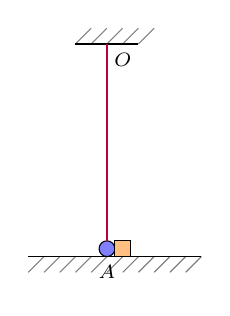
\begin{tikzpicture}[font=\scriptsize]
    \filldraw[fill=blue!50] (0,-.1) circle(.1);
    \filldraw[fill=orange!50] (.1,-.2) rectangle(.3,0);
    \foreach \x in {-1,-.8,...,1}
        \draw[gray] (\x,-.4)--++(.2,.2);
    \draw (-1,-0.2)--(1.2,-0.2);
    \foreach \x in {-.4,-.2,...,.4}
        \draw[gray] (\x,2.5)--++(.2,.2);
    \draw (-.4,2.5)--(.4,2.5);
    \draw[purple] (0,2.5)--(0,0);
    \node at(.2,2.3){\(O\)};
    \node at(0,-.4){\(A\)};
    \end{tikzpicture}
    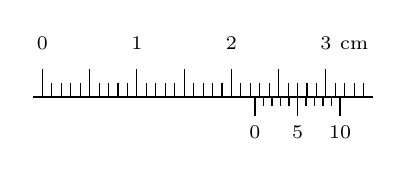
\begin{tikzpicture}[scale=1.2,font=\scriptsize]
		\draw (-2.8,0)--(.8,0);
		\foreach \x/\n in {.3/3,-.7/2,-1.7/1,-2.7/0}
			\node at(\x,.4)[above]{\(\n\)};
		\foreach \x in {.3,-.2,...,-2.7}
			\draw (\x,.3)--(\x,.15);
		\foreach \x in {.7,.6,...,-2.7}
				\draw (\x,.15)--(\x,0);
		\foreach \x in {-.45,-.36,...,.45}
			\draw (\x,-.1)--(\x,0);
		\foreach \x/\n in {-.45/0,0/5,.45/10}
			\draw (\x,-.2)node[below]{\(\n\)}--(\x,-.1);
		\node at(.6,.4)[above]{\qty{}{cm}};
	\end{tikzpicture}
\end{figure}

(1)用游标卡尺测量摆球直径，如图乙所示，摆球的直径\(d =\)\underline{\hbox to 4em{}}\,\qty{}{cm}。

(2)将摆球向左拉起，使摆线与竖直方向的夹角为\(\alpha\)，在\(A\)点放置一小滑块，释放摆球，摆球运动到最低位置时与滑块发生正碰，而后摆球向右摆动，摆线与竖直方向的最大角度为\(\beta\)，滑块向右运动的最大位移为\(x\)，已知滑块与水平面之间的动摩擦因数为\(\mu\)，滑块的质量为\(M\)，摆球的质量为\(m\)（\(m > M\)），摆线长为\(L_0\)，摆球的直径为\(d\)，则摆球与滑块碰撞后瞬间滑块的速度大小为\underline{\hbox to 10em{}}。

(3)当在误差允许的范围内，满足\underline{\hbox to 10em{}}时，说明摆球与滑块碰撞过程动量守恒。（填写利用已知量表示的最简式）
\begin{answer}
    （1）（2）（3）
\end{answer}